\chapter*{Appendices}
\addcontentsline{toc}{chapter}{Appendices}

\section*{Appendix A}
\addcontentsline{toc}{section}{Appendix A}

\begin{landscape}
\begin{figure}[H]
	\centering
	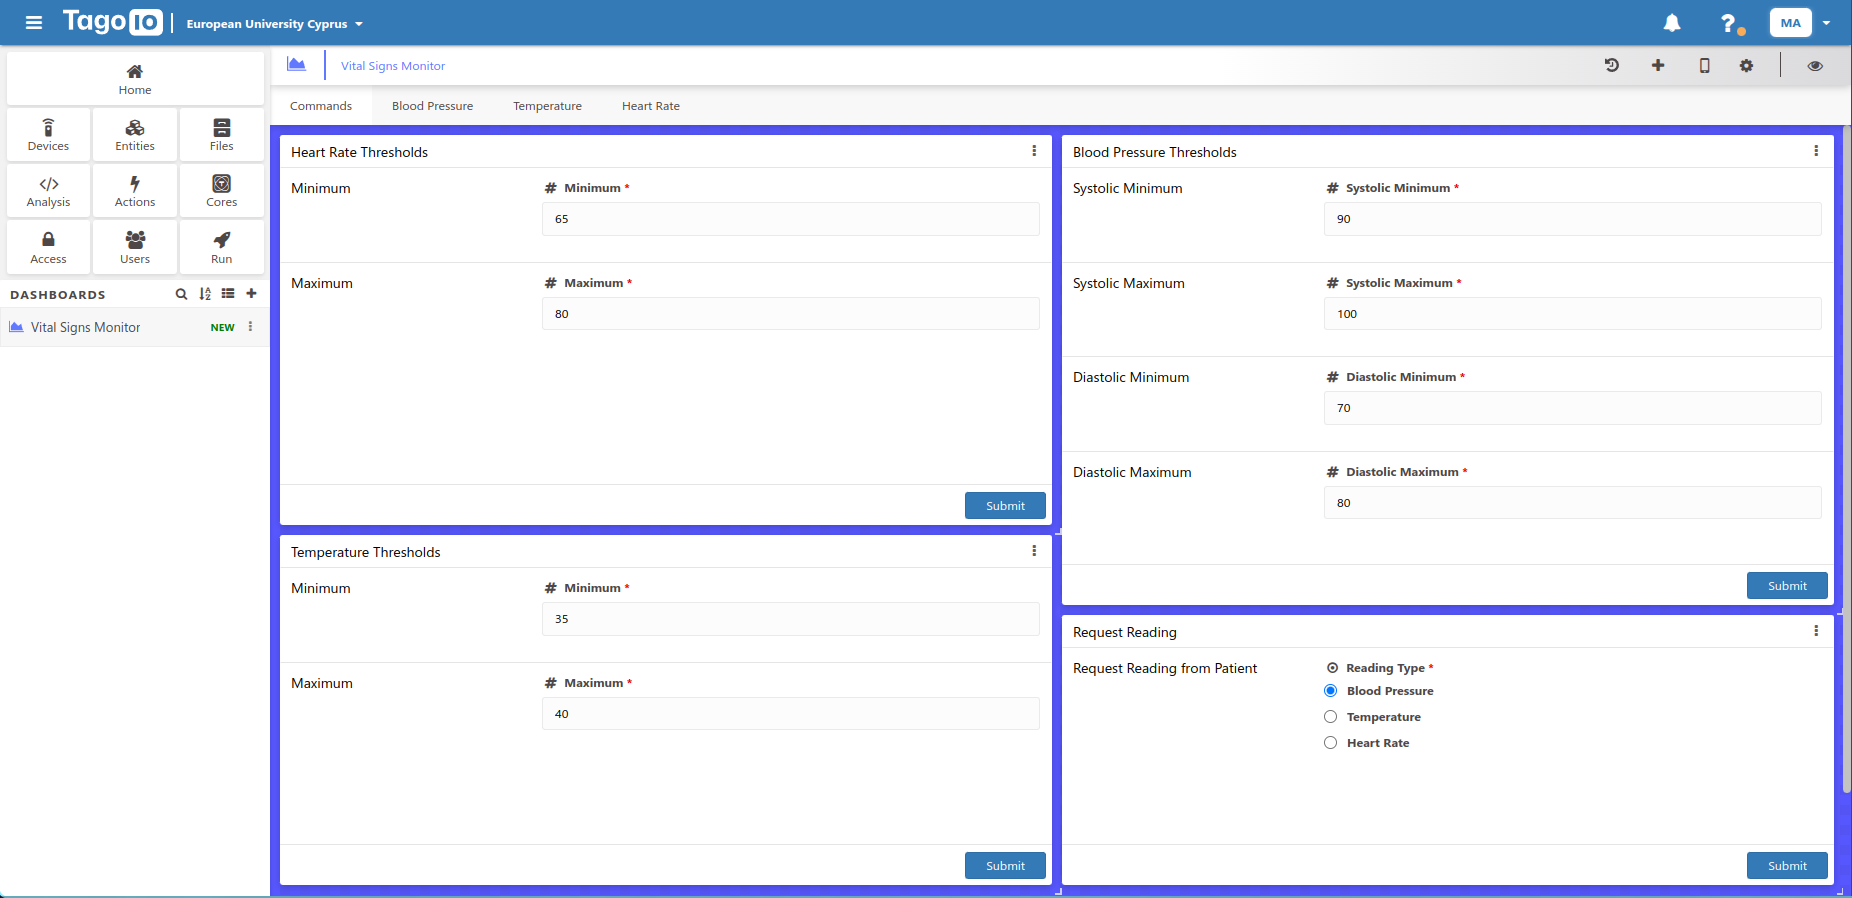
\includegraphics[width=\linewidth]{images/tagoio_dashboard_cmds}
	\caption{TagoIO dashboard: Commands pannel for remote requests and thresholds setting}
	\label{appendix:tagoio_commands}
\end{figure}
\end{landscape}

\newpage
\begin{landscape}
\begin{figure}[H]
	\centering
	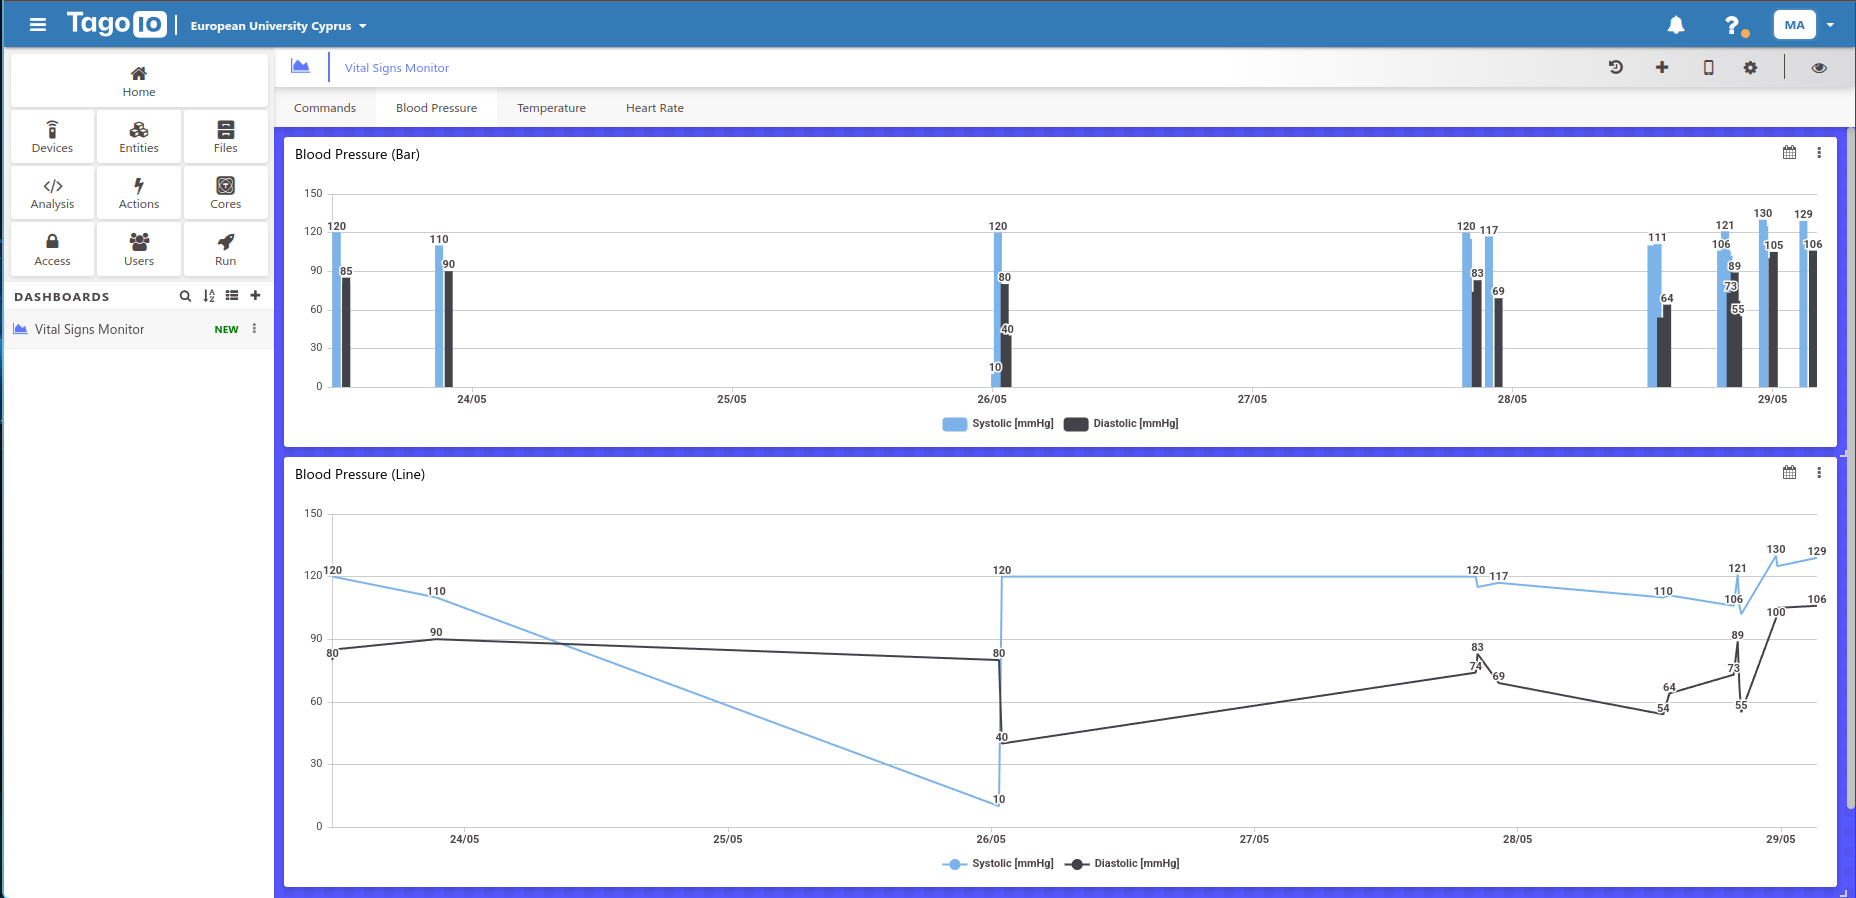
\includegraphics[width=\linewidth]{images/tagoio_dashboard_bp}
	\caption{TagoIO dashboard: Blood pressure visualisation panel}
	\label{appendix:tagoio_bp}
\end{figure}
\end{landscape}

\newpage
\begin{landscape}
\begin{figure}[H]
	\centering
	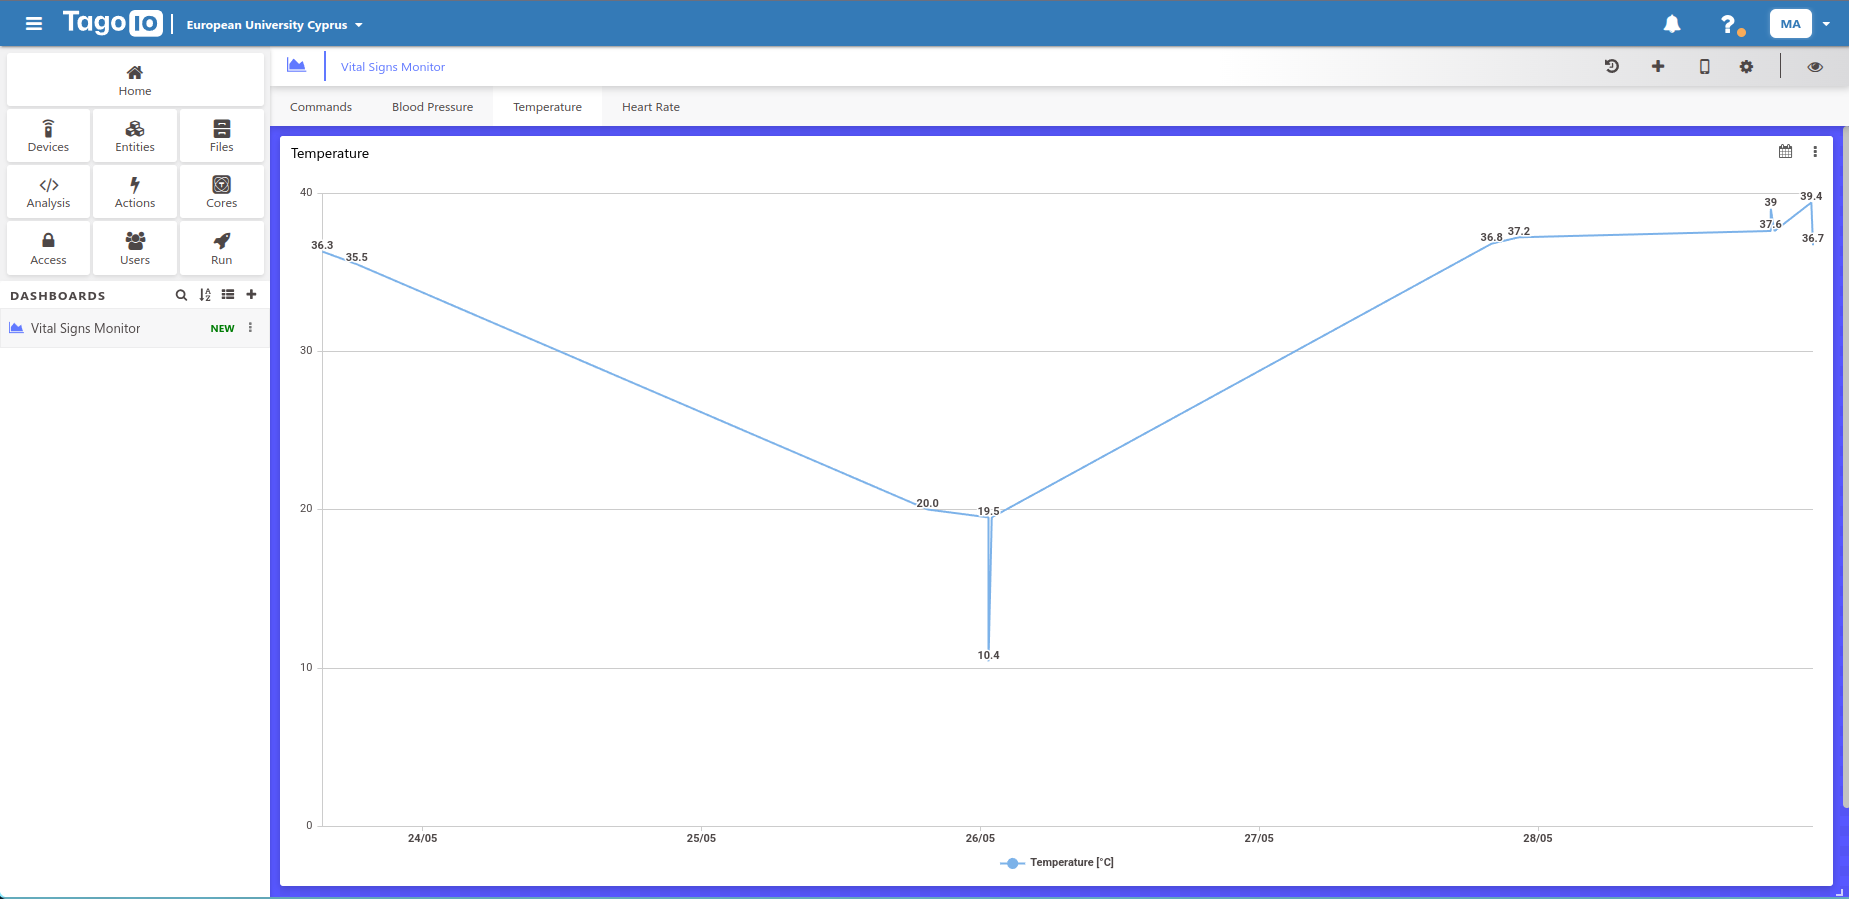
\includegraphics[width=\linewidth]{images/tagoio_dashboard_temp}
	\caption{TagoIO dashboard: Temperature visualisation panel}
	\label{appendix:tagoio_temp}
\end{figure}
\end{landscape}

\newpage
\begin{landscape}
\begin{figure}[H]
	\centering
	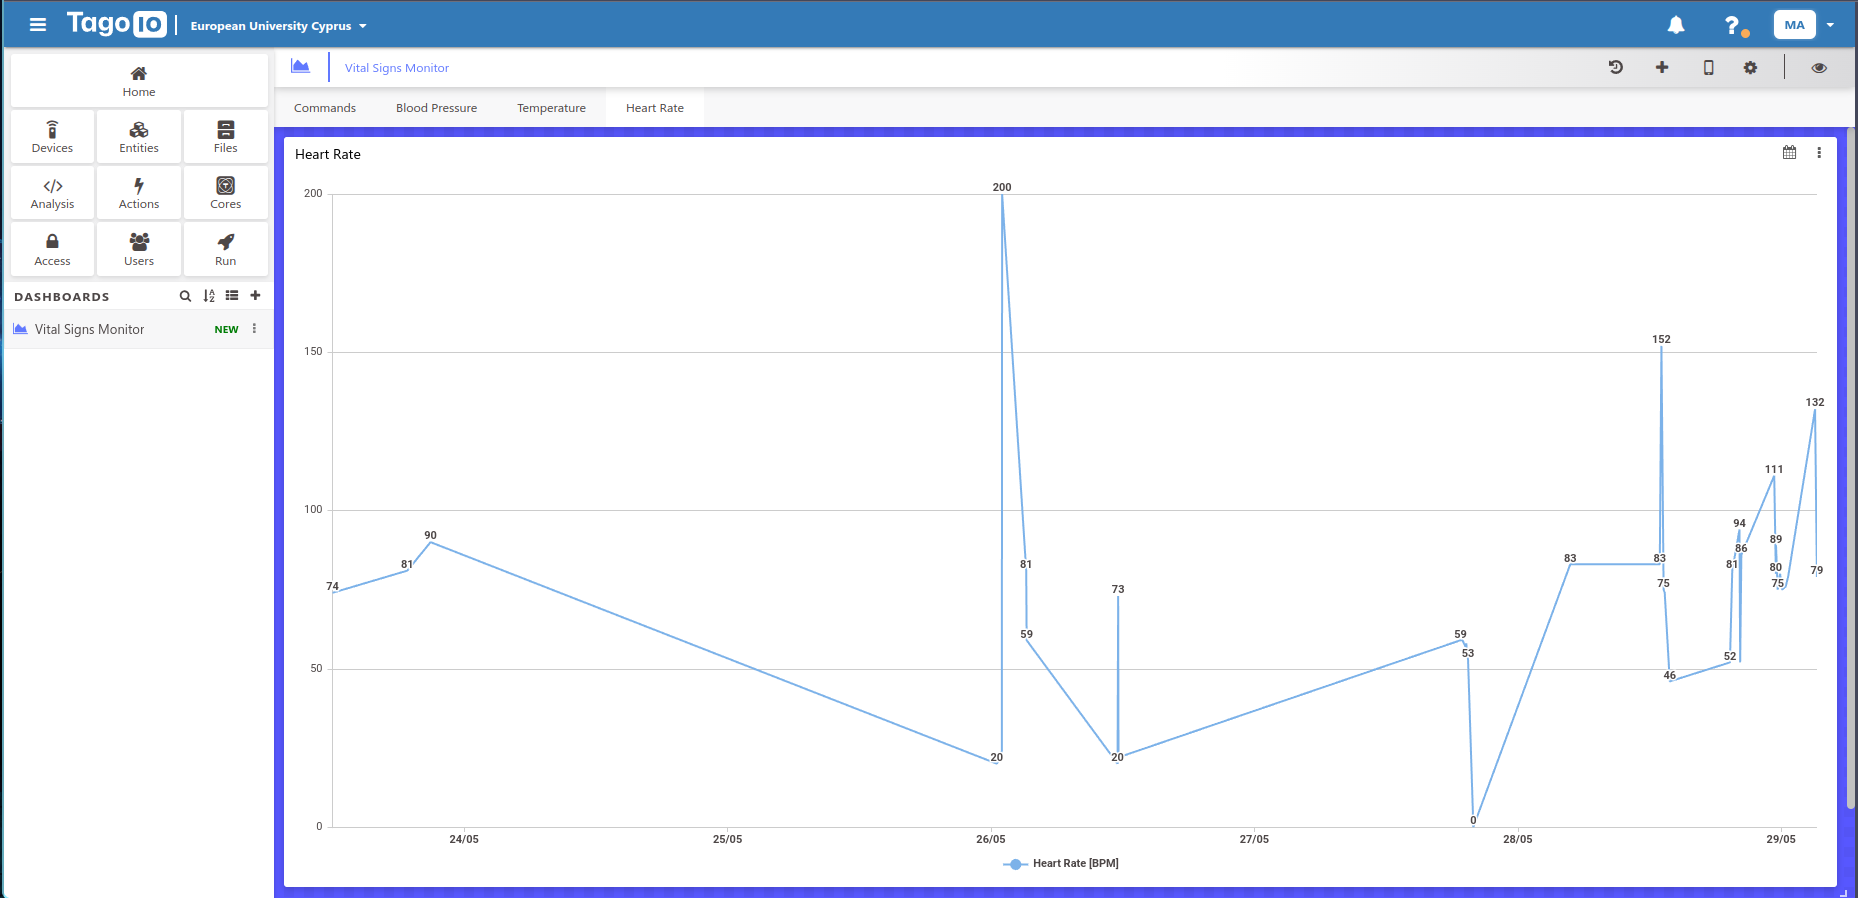
\includegraphics[width=\linewidth]{images/tagoio_dashboard_hr}
	\caption{TagoIO dashboard: Heart rate visualisation panel}
	\label{appendix:tagoio_hr}
\end{figure}
\end{landscape}

\newpage
\begin{landscape}
\begin{figure}[H]
	\centering
	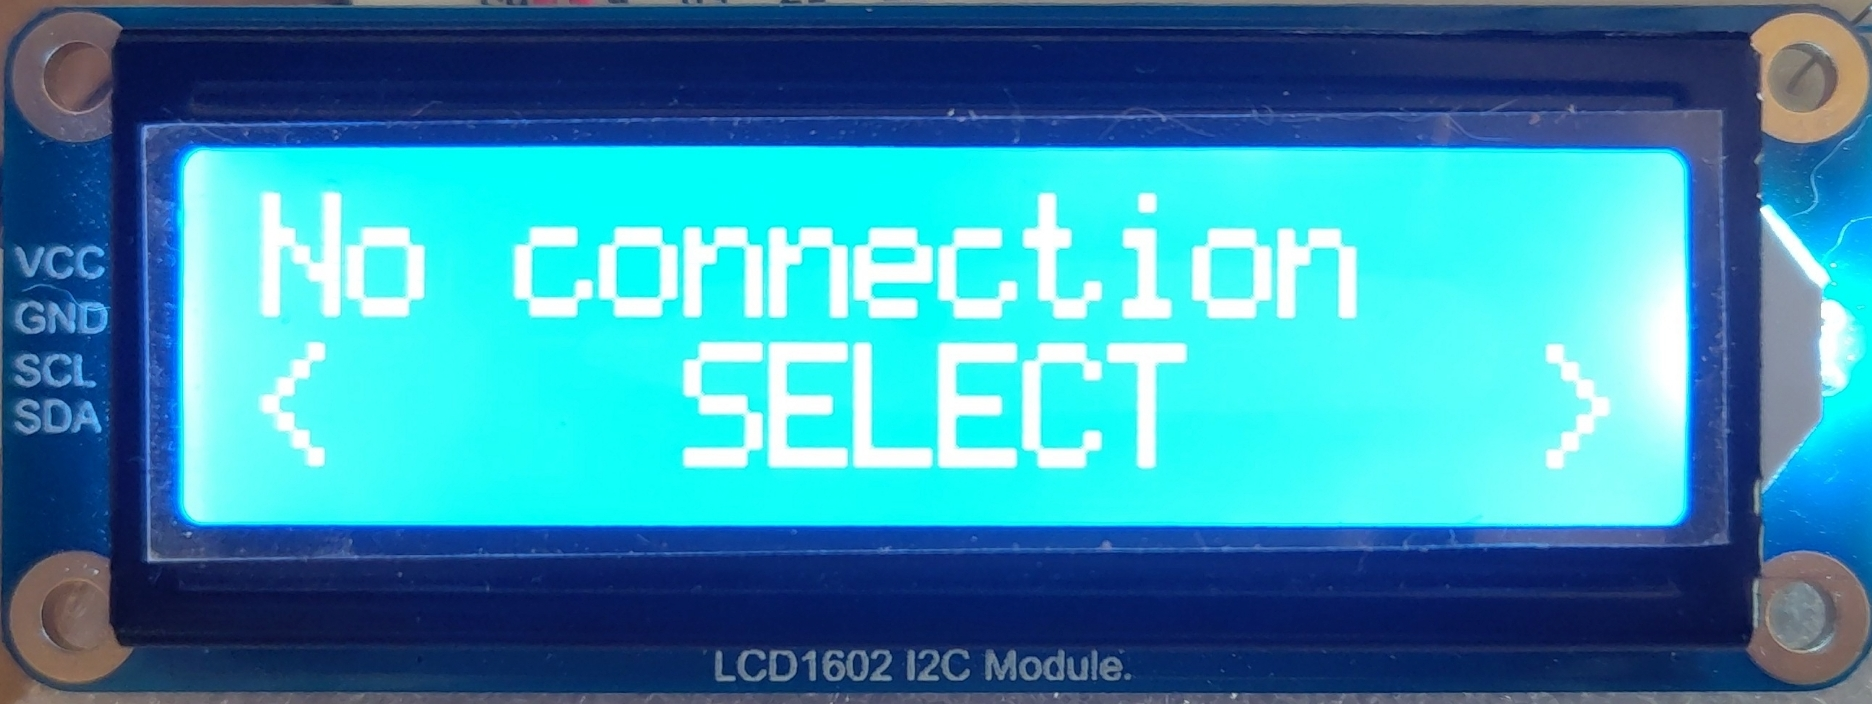
\includegraphics[width=\linewidth]{images/device_ui_disconnected.jpg}
	\caption{Full-size view of device LCD in DISCONNECTED state}
	\label{appendix:ui_disconnected}
\end{figure}
\end{landscape}

\newpage
\begin{landscape}
\begin{figure}[H]
	\centering
	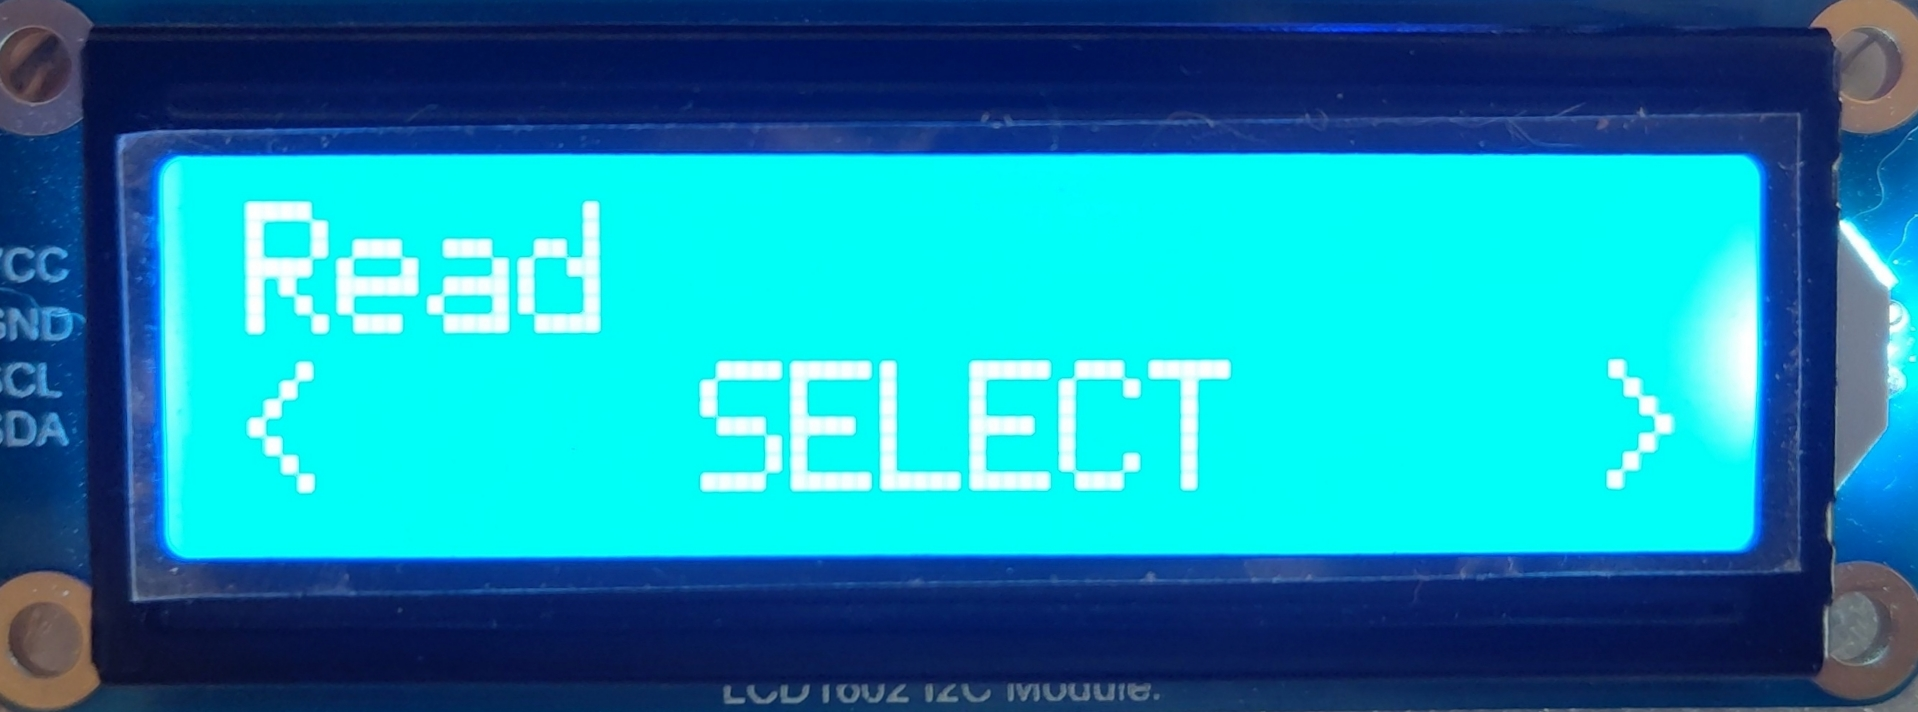
\includegraphics[width=\linewidth]{images/device_ui_connected.jpg}
	\caption{Full-size view of device LCD in CONNECTED state}
	\label{appendix:ui_connected}
\end{figure}
\end{landscape}

\newpage
\begin{landscape}
\begin{figure}[H]
	\centering
	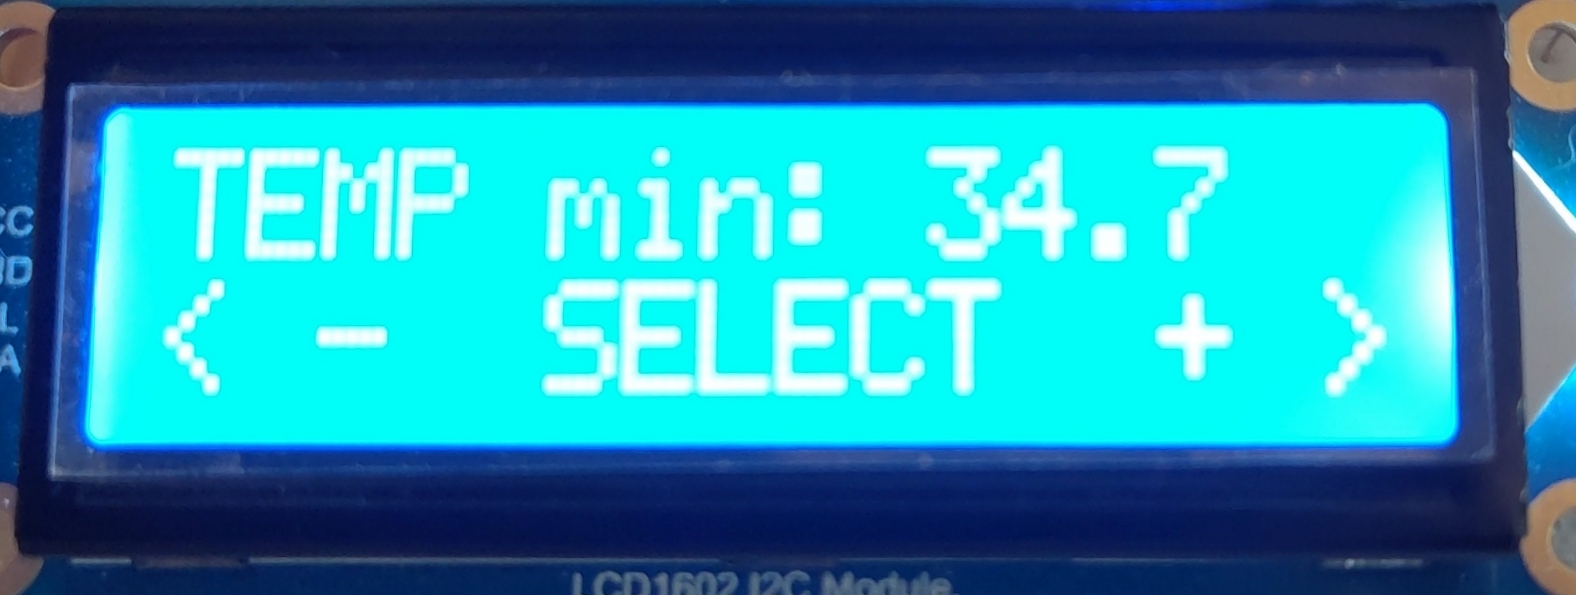
\includegraphics[width=\linewidth]{images/device_ui_set_temp.jpg}
	\caption{Full-size view of device LCD in SETUP\_TEMP configuration substate}
	\label{appendix:ui_setup_temp}
\end{figure}
\end{landscape}

% \newpage
\begin{figure}[H]
	\centering
	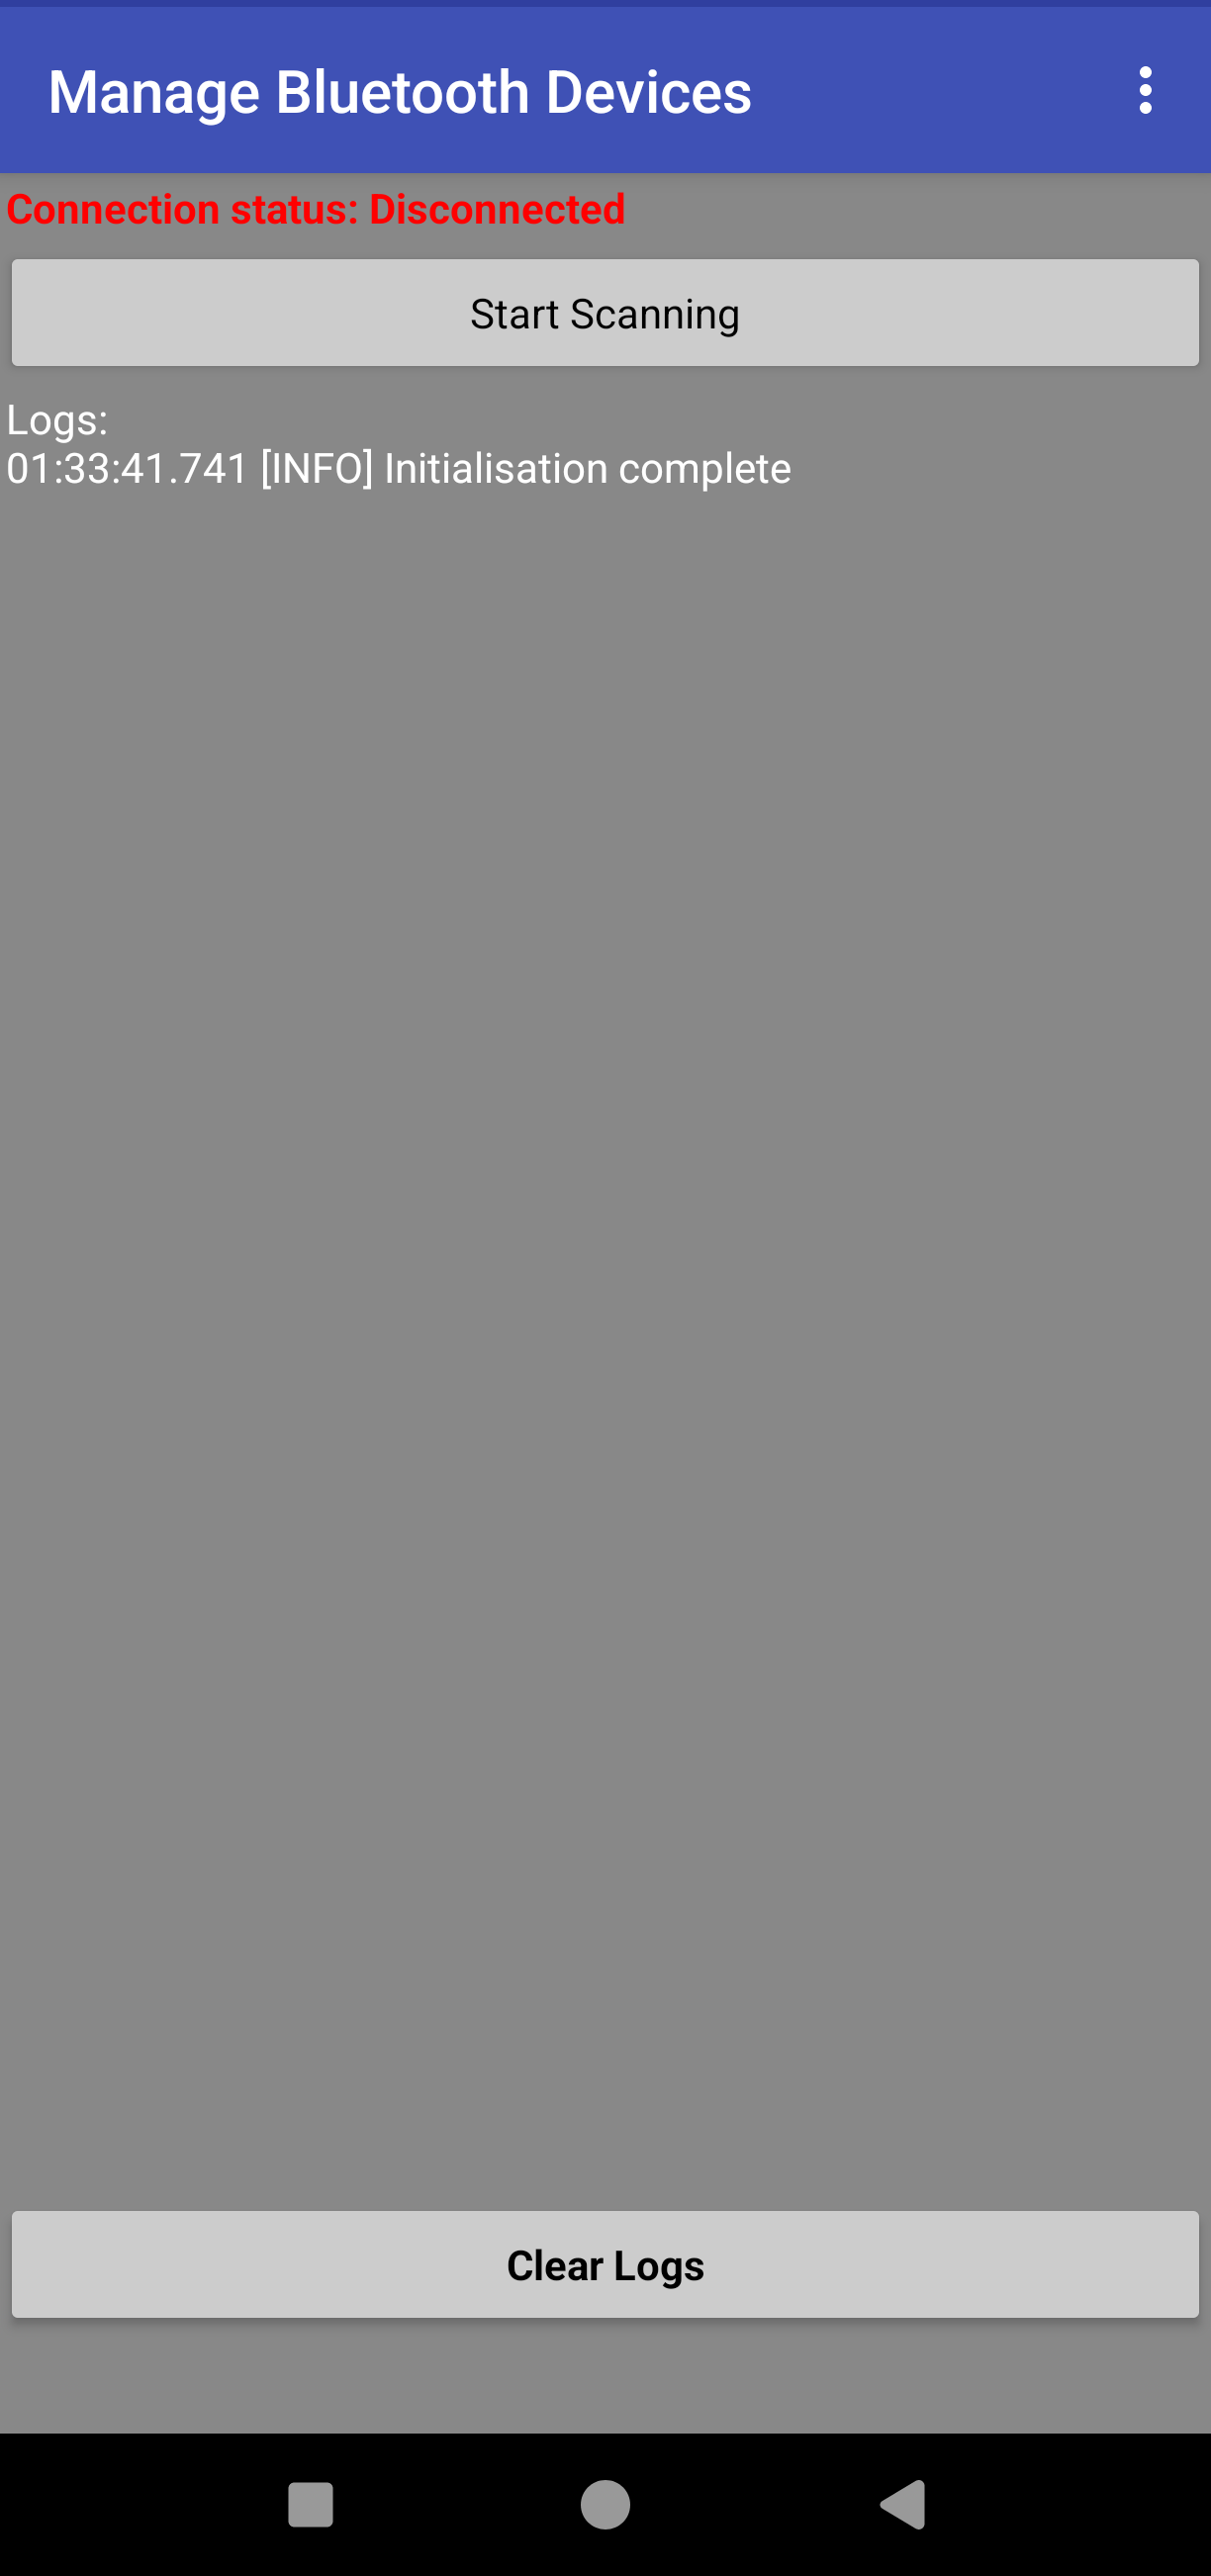
\includegraphics[width=0.7\textwidth]{images/app_ui_main_disconnected}
	\caption{App UI: First screen visible when starting the app}
	\label{appendix:app_ui_disconnected}
\end{figure}

\newpage
\begin{figure}[H]
	\centering
	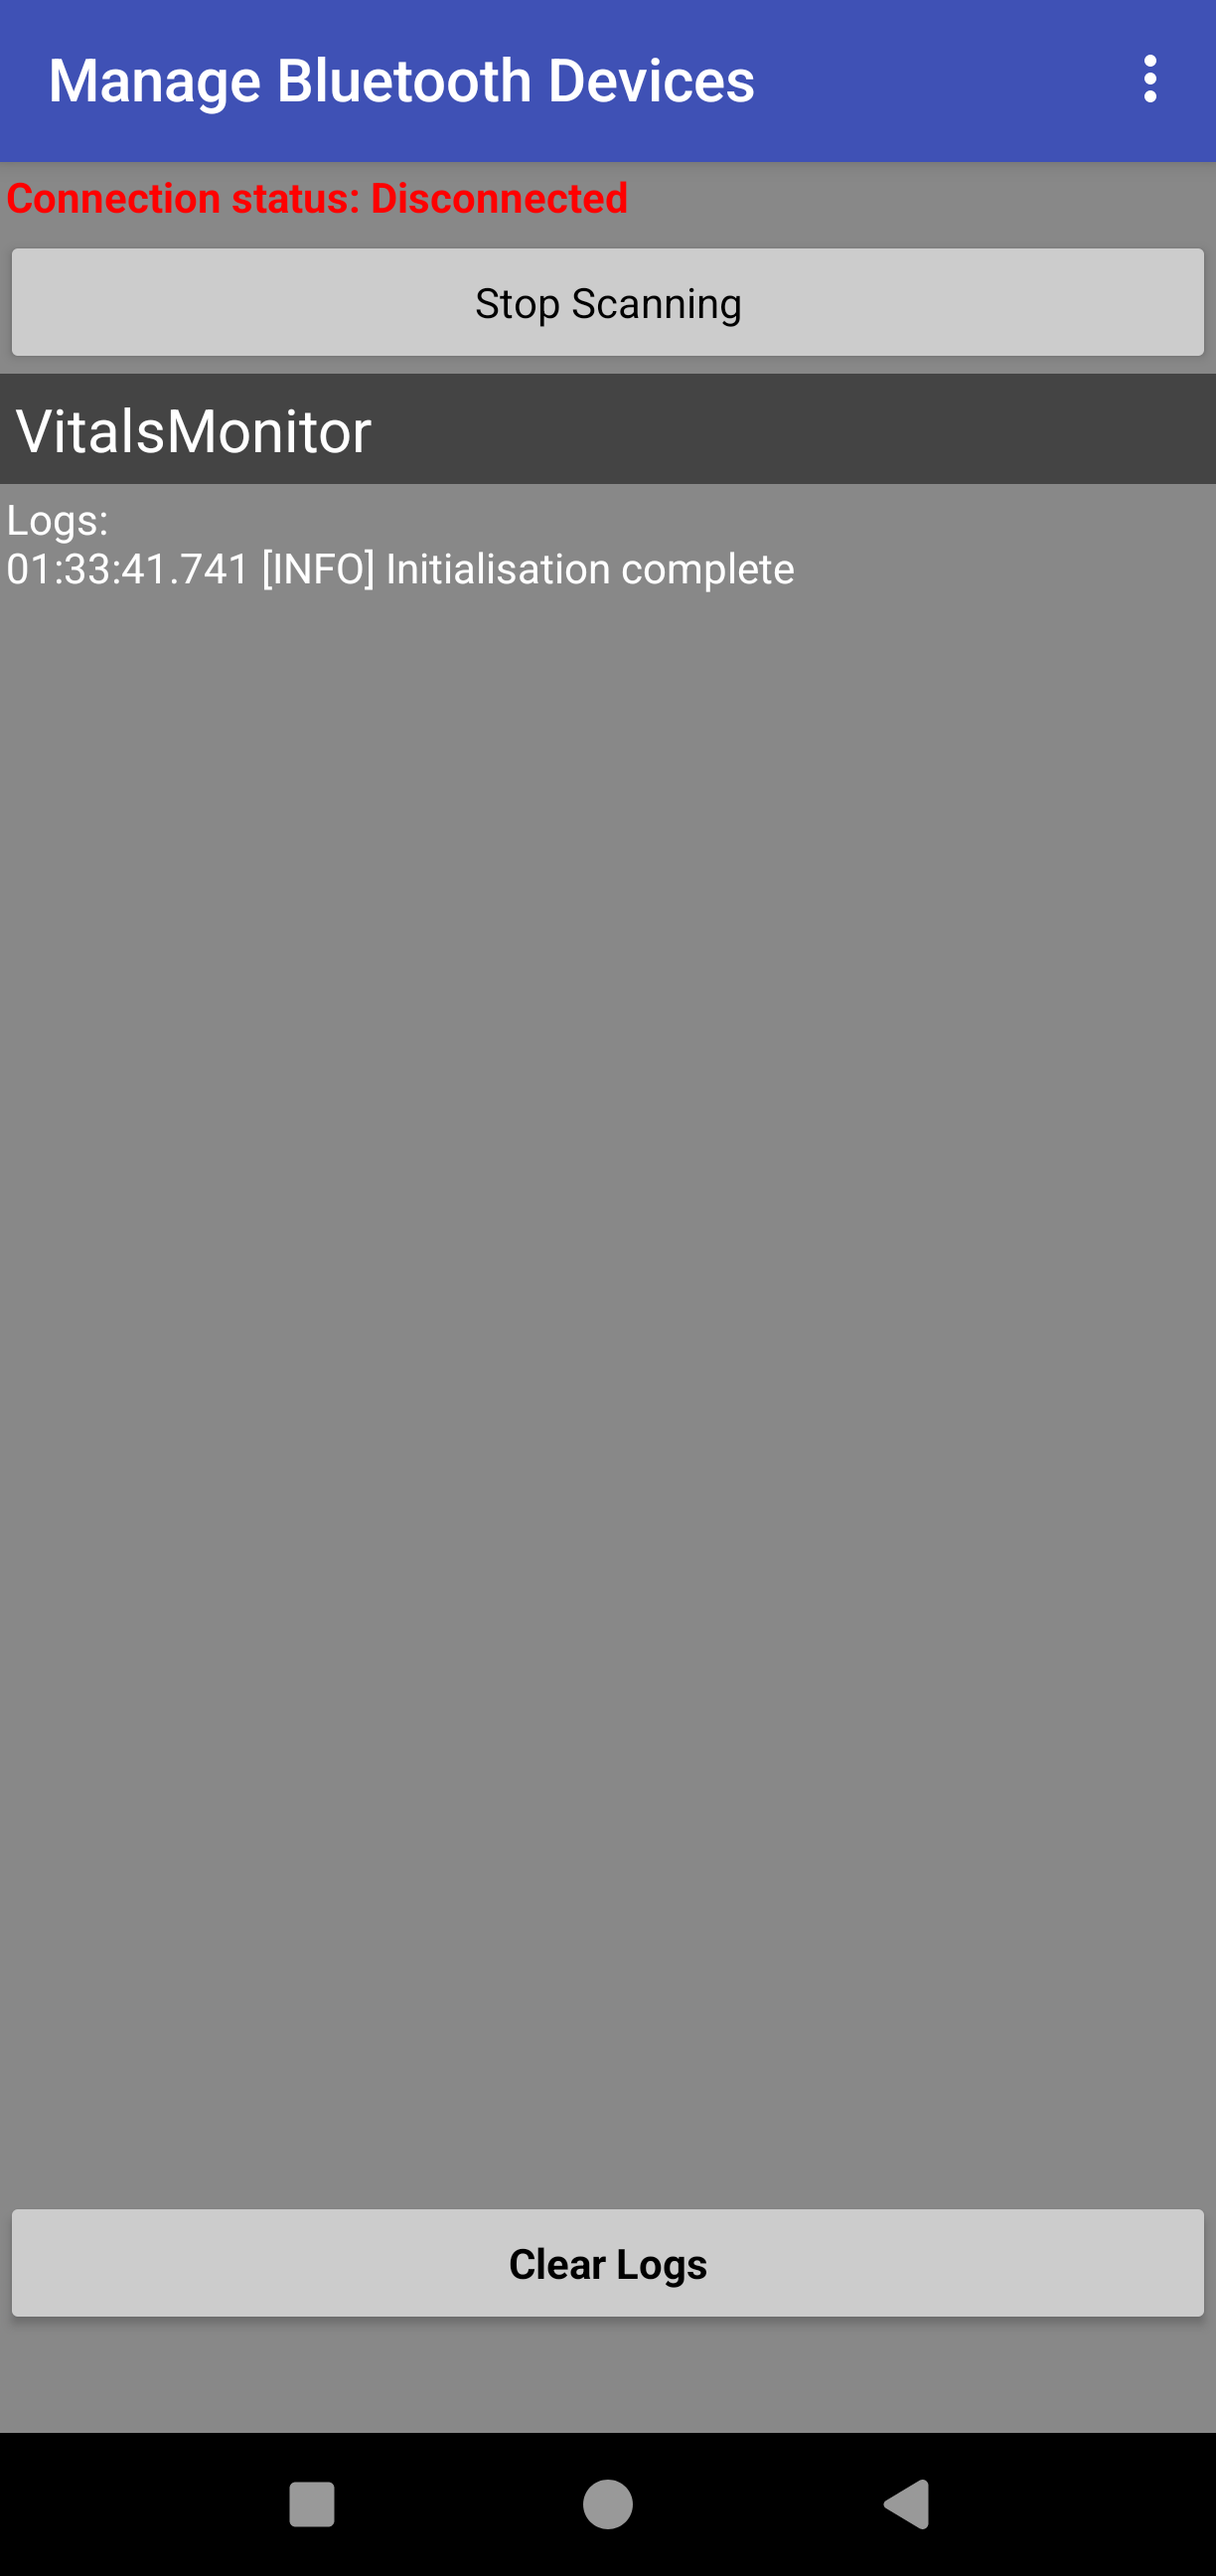
\includegraphics[width=0.7\textwidth]{images/app_ui_main_scanning}
	\caption{App UI: Screen when scanning for available Bluetooth devices}
	\label{appendix:app_ui_scanning}
\end{figure}

\newpage
\begin{figure}[H]
	\centering
	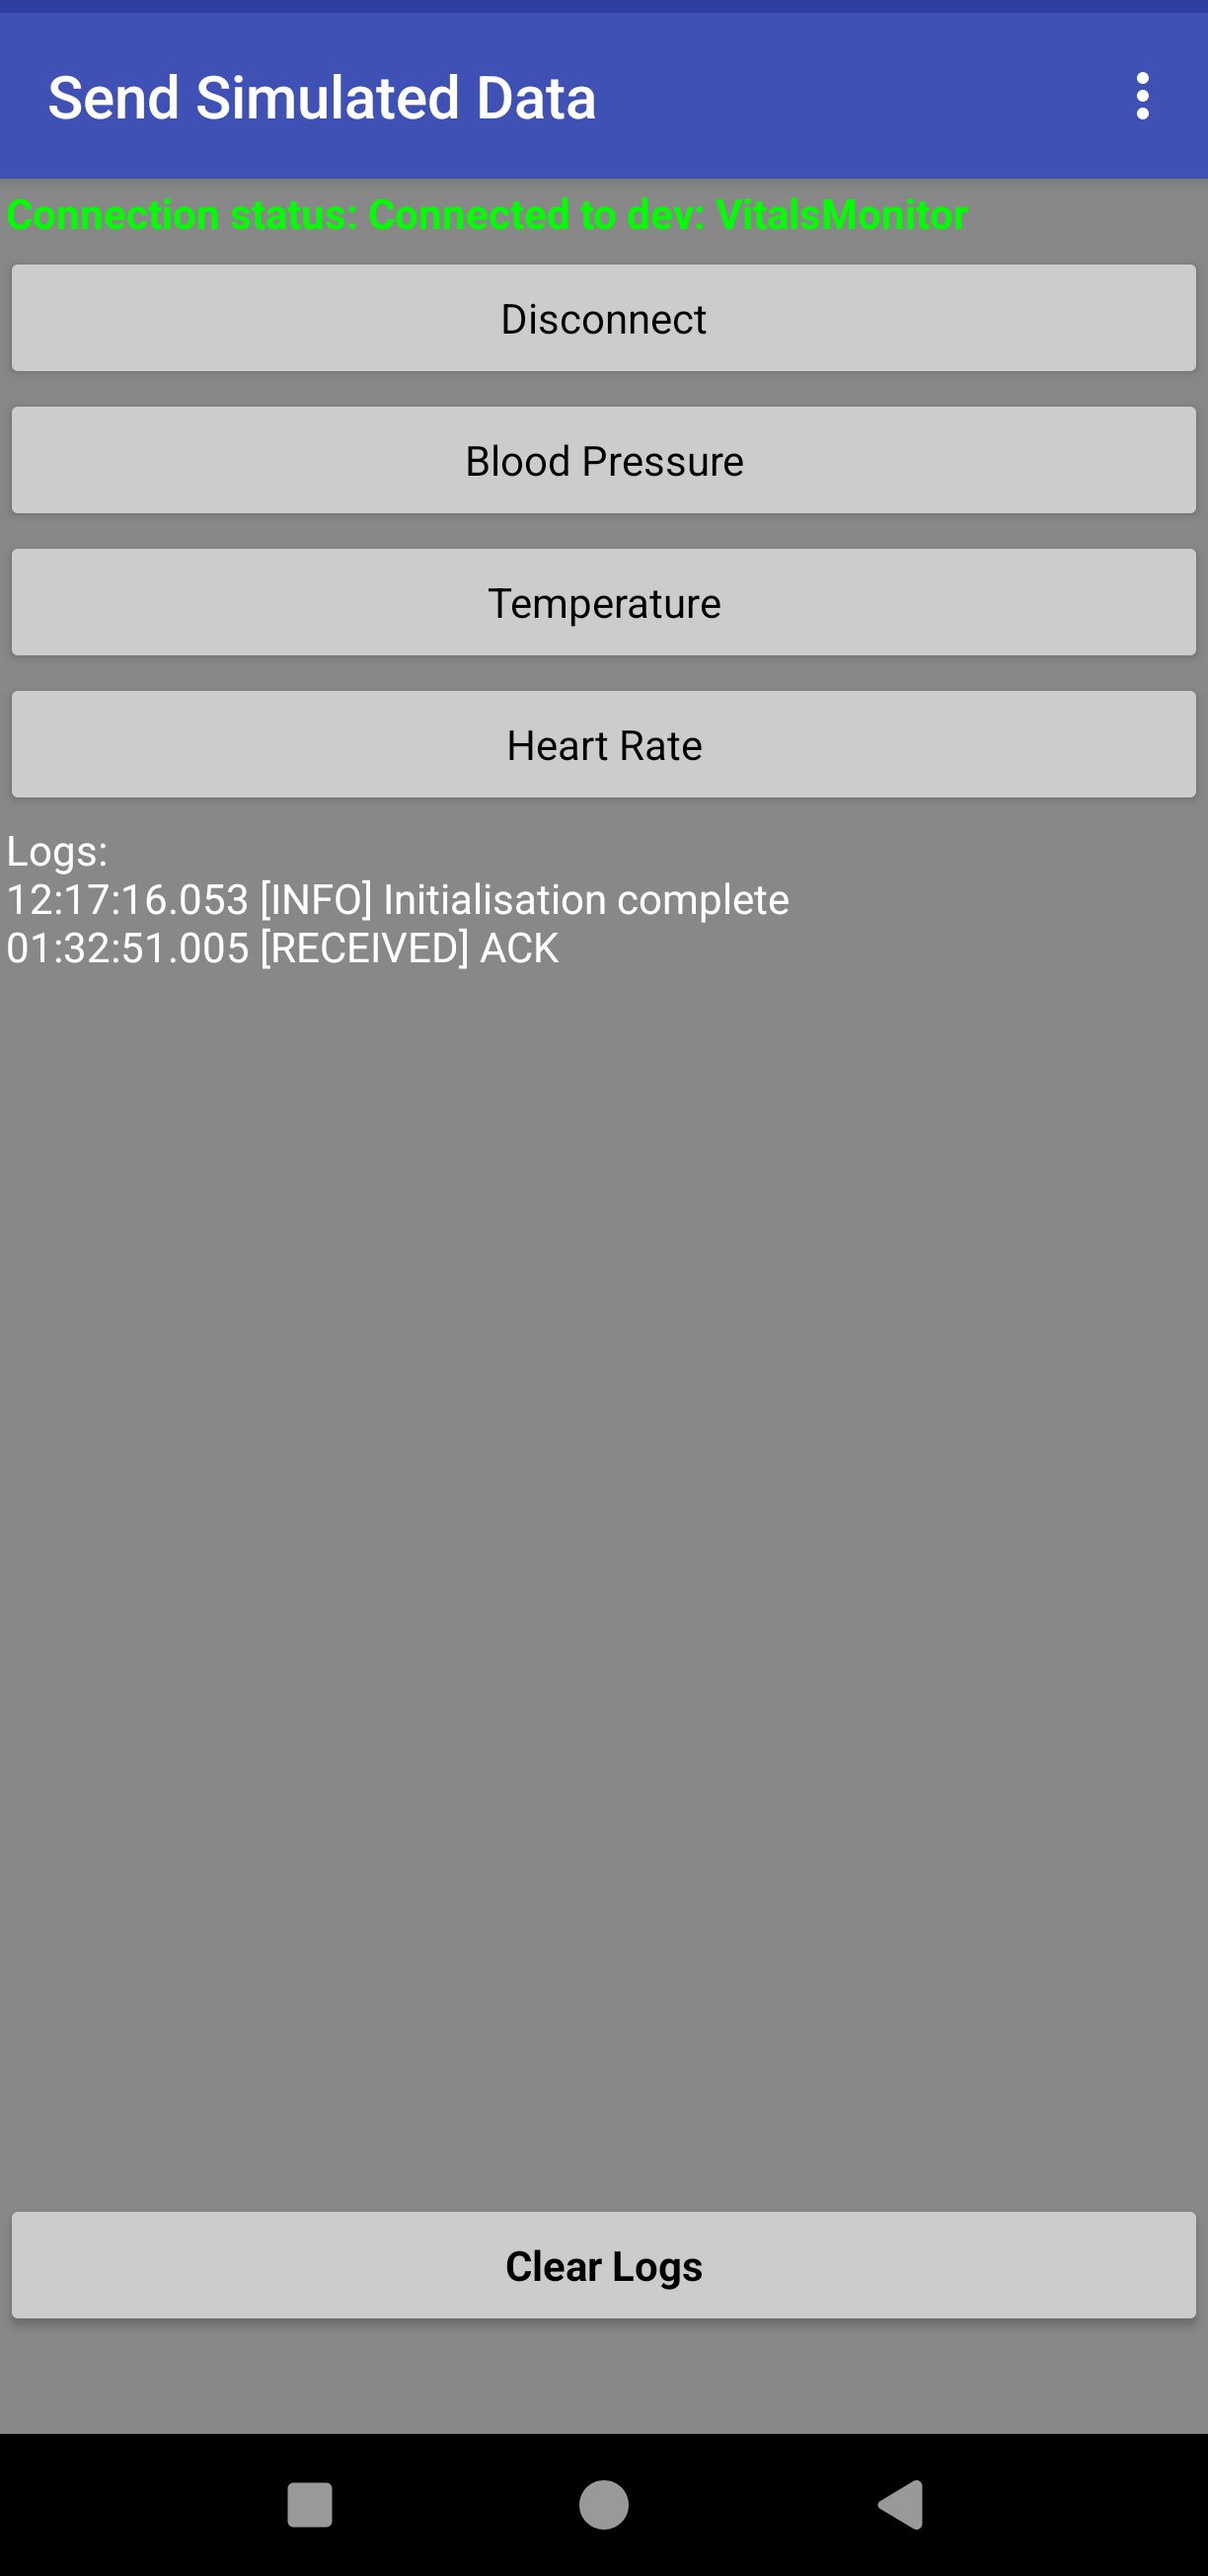
\includegraphics[width=0.7\textwidth]{images/app_ui_main_connected}
	\caption{App UI: Screen that is shown after a successful connection is established}
	\label{appendix:app_ui_connected}
\end{figure}

\newpage
\begin{figure}[H]
	\centering
	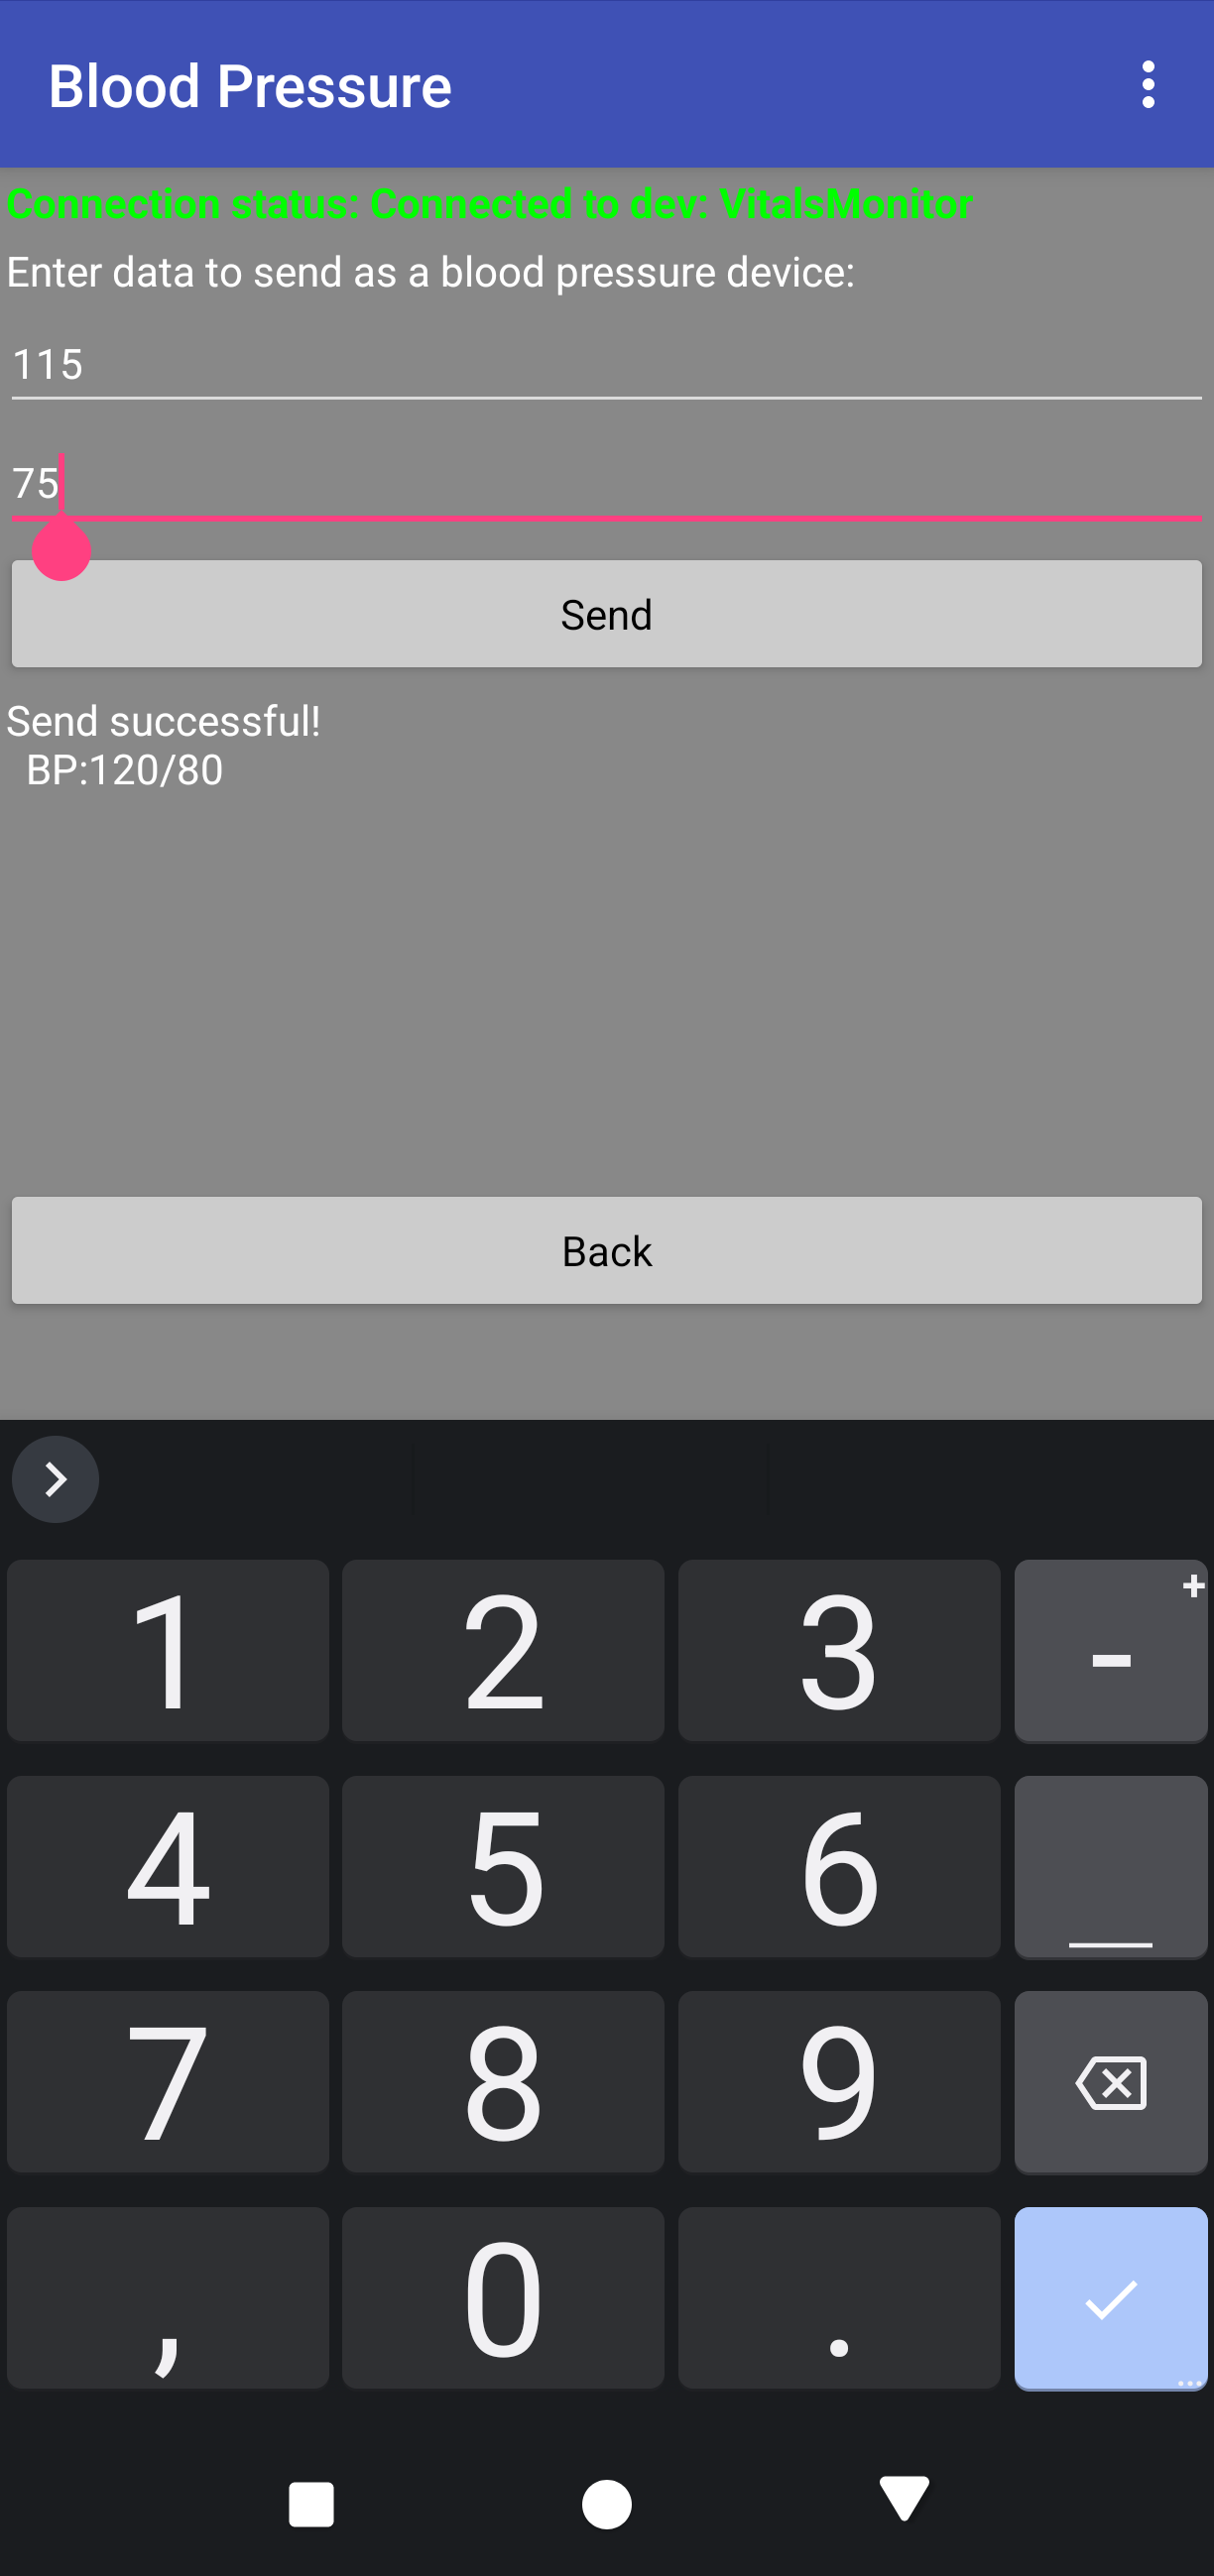
\includegraphics[width=0.7\textwidth]{images/app_ui_send_bp}
	\caption{App UI: Screen to send blood pressure data}
	\label{appendix:app_ui_bp}
\end{figure}

\newpage
\begin{figure}[H]
	\centering
	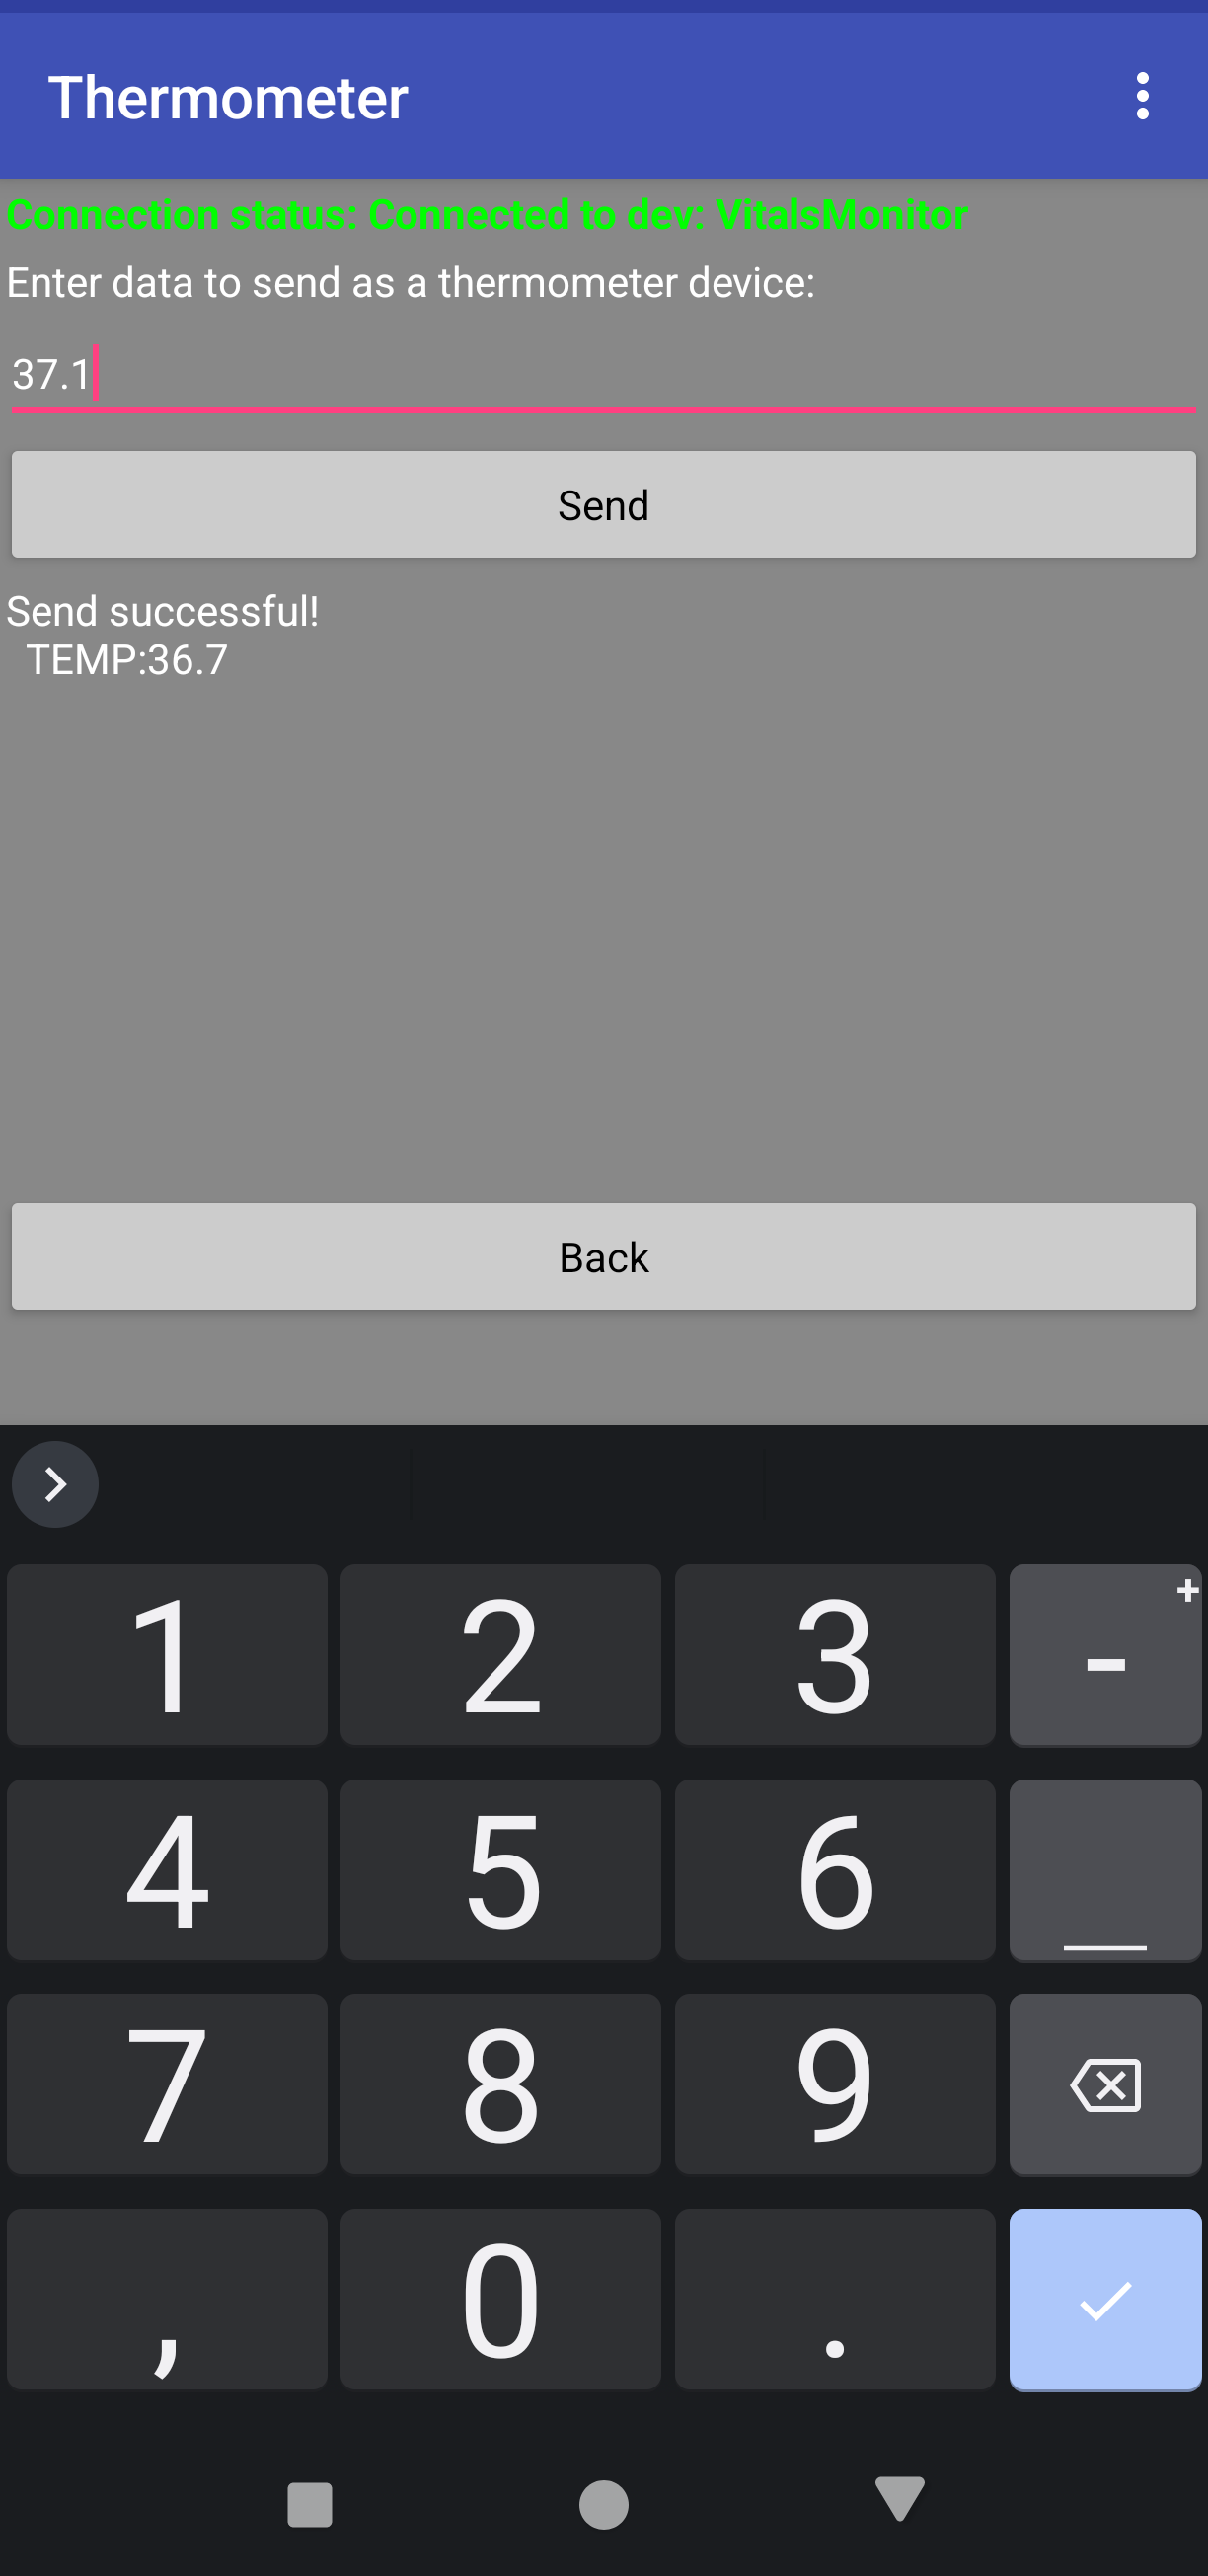
\includegraphics[width=0.7\textwidth]{images/app_ui_send_temp}
	\caption{App UI: Screen to send temperature data}
	\label{appendix:app_ui_temp}
\end{figure}

\newpage
\begin{figure}[H]
	\centering
	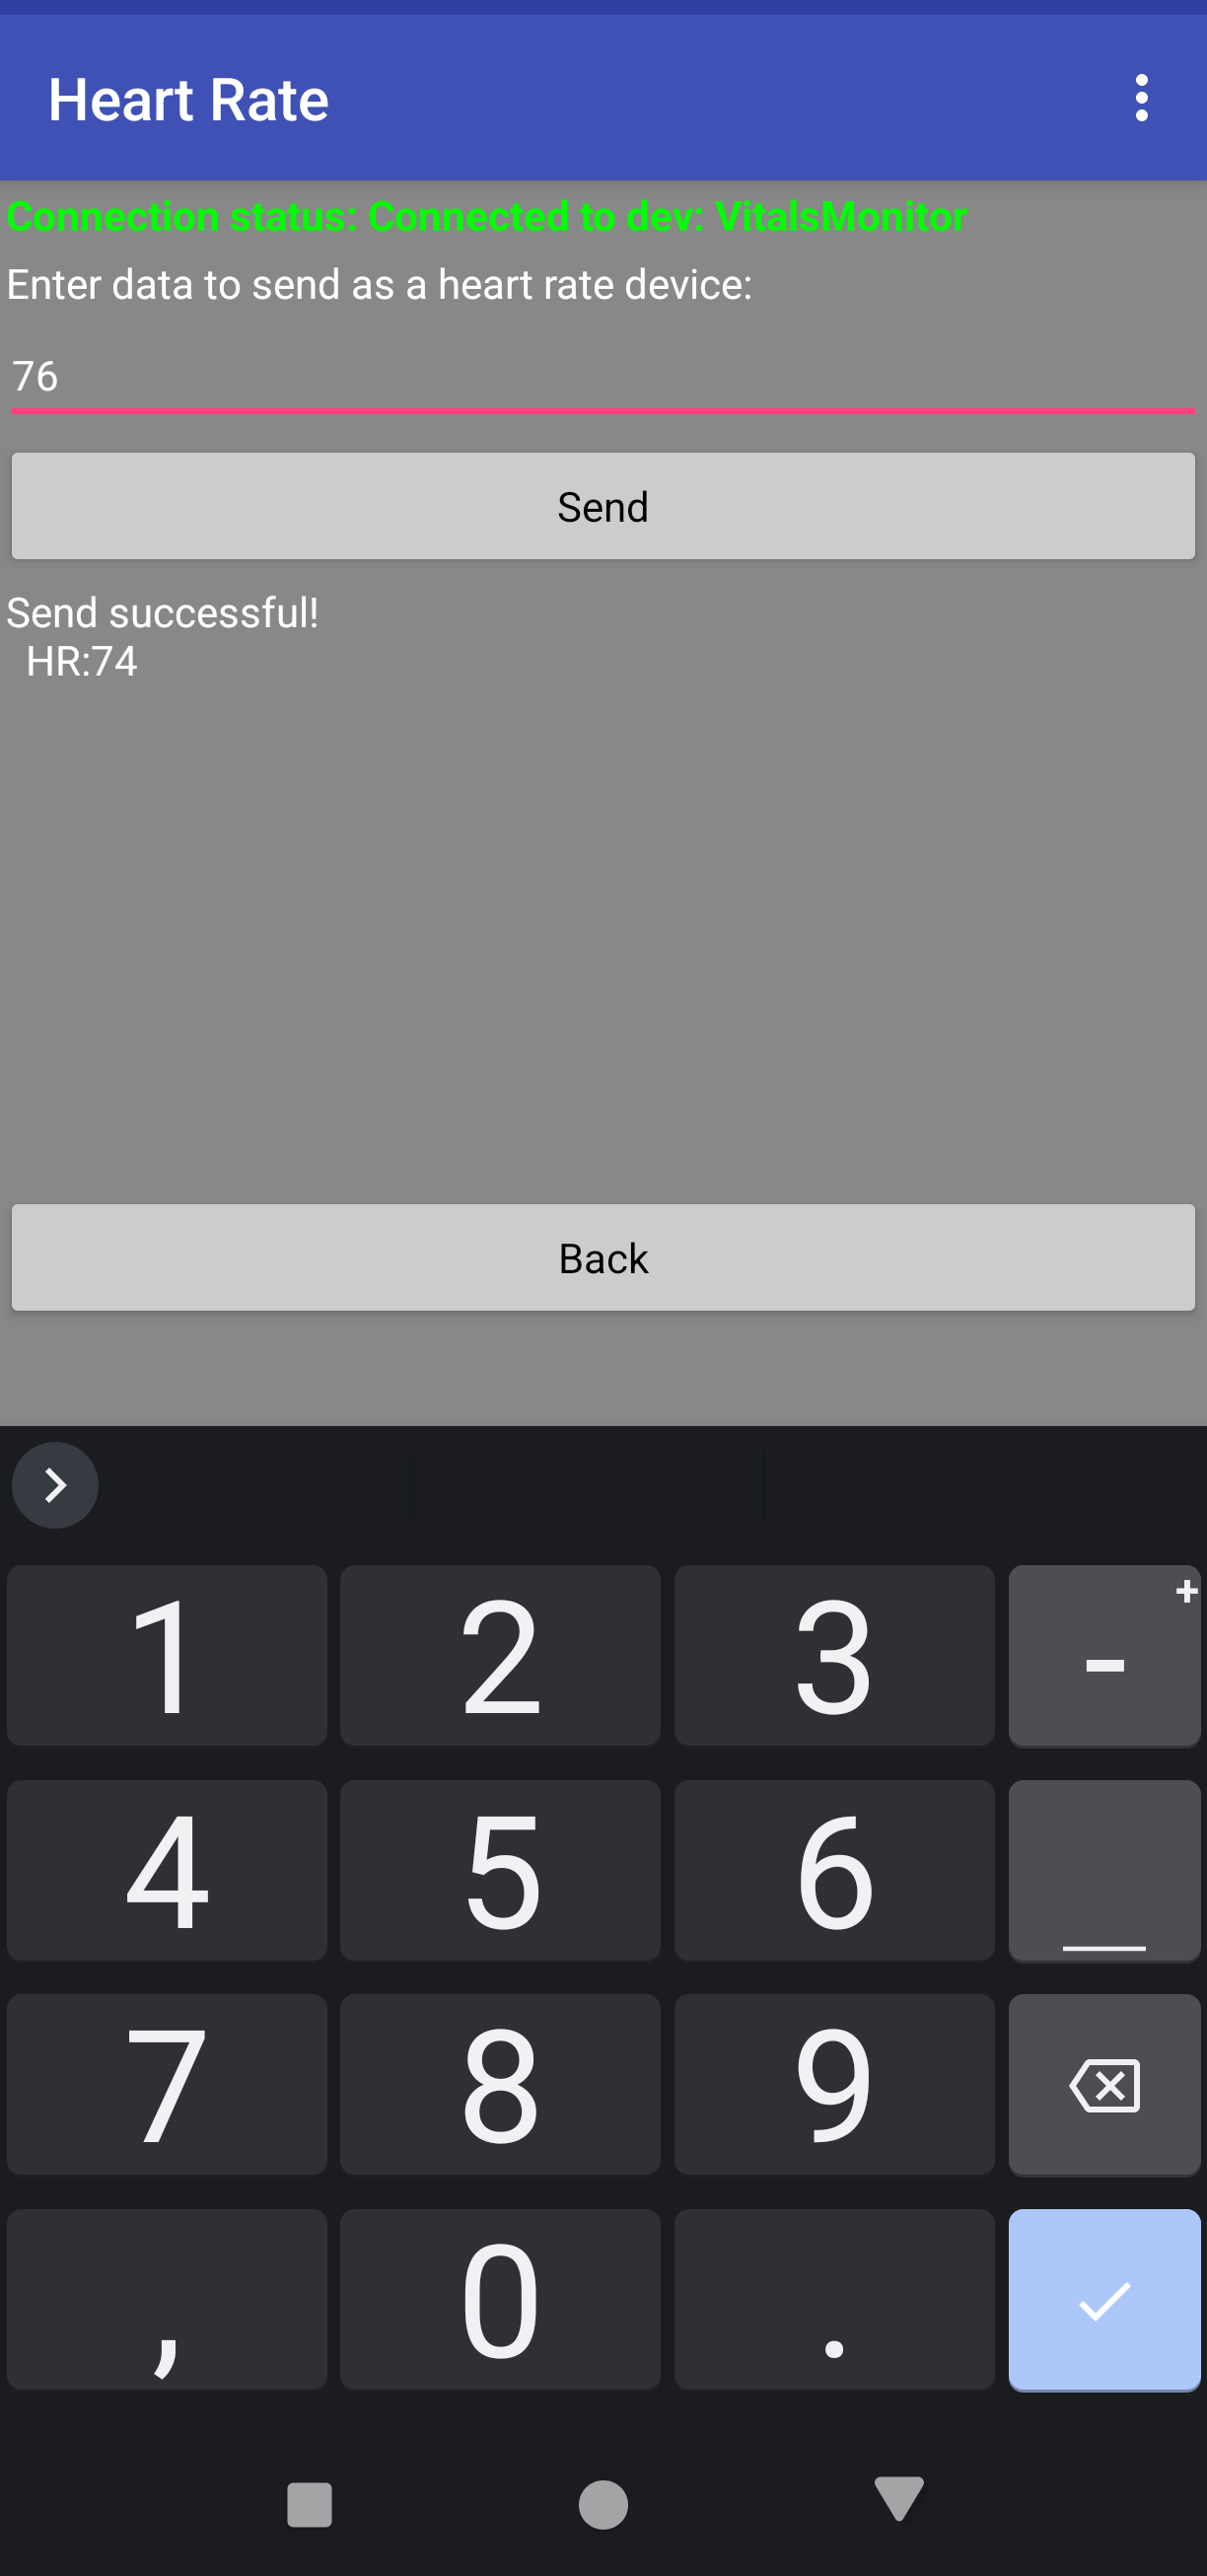
\includegraphics[width=0.7\textwidth]{images/app_ui_send_hr}
	\caption{App UI: Screen to send heart rate data}
	\label{appendix:app_ui_hr}
\end{figure}

% \newpage
% \section*{Appendix B}
% \addcontentsline{toc}{section}{Appendix B}
% Write a few words about the contents of the appendix
